\documentclass[a4paper,12pt]{report}
\usepackage{fancyhdr}
\pagestyle{fancy}
\usepackage{amsfonts}
\usepackage{amsmath}
\usepackage{tikz}
\usepackage[utf8]{inputenc}
\usepackage[serbianc]{babel}
\usepackage{titling}
\usepackage{caption}
\usepackage{subcaption}
\usepackage{titlesec}
\usepackage{fancyhdr}
\usepackage[bookmarks]{hyperref}

\usepackage[margin=2.5cm]{geometry}
\addtolength{\hoffset}{0.5cm}
\addtolength{\textwidth}{-0.5cm}

\fancyheadoffset{1 cm}

\setlength\parindent{0pt}

\titleformat
{\chapter} % command
[display] % shape
{\bfseries\Large\itshape} % format
{Glava \ \thechapter} % label
{0.5ex} % sep
{
    \rule{\textwidth}{1pt}
    \vspace{1ex}
    \centering
} % before-code
[
\vspace{-0.5ex}%
\rule{\textwidth}{0.3pt}
] % after-code

\pagestyle{fancy}
\fancyhf{}
\rhead{Glava \ \thechapter}
\lhead{\thesection}
\cfoot{\thepage}

\captionsetup[figure]{name=Slika}


\begin{document}
\renewcommand*\contentsname{ }

\begin{titlepage}
\begin{center}

	\textbf{\Large Univerzitet u Beogradu}\\[0.5cm]
	
	{\large Matematički fakultet}\\[6cm]
	
	\textsc{\huge grupni studentski rad}\\[0.5cm]
	
	\textbf{\Large Informacioni sistem izdavaštva časopisa}\\[10cm]

	\begin{tabular}{|l|l|}
  		\hline
	    Studenti: & Ozren Demonja \\ \cline{2-2}
	              & Stefan Maksimović \\ \cline{2-2}
	              & Marko Crnobrnja \\ \hline
	    Predmet: & Informacioni sistemi (R271) \\ \hline
	    Školska godina: & 2016/2017. \\ \hline
	    Profesor: & Dr Saša Malkov	 \\ \hline
	    Datum &  \\ \hline
	\end{tabular}

\newpage
\end{center}
\end{titlepage}

\begin{center}
	\textbf{\large SADRŽAJ}
\end{center}
\tableofcontents 
\newpage

\chapter{Uvod}

 Ovaj rad se bavi modeliranjem informacionog sistema Izdavaštva jednog časopisa. Modelira se deo sistema koji se odnosi na stvaranje sadržaja časopisa i njegovo ob\-ja\-vlji\-va\-nje. Razmatrani časopis ima pisano kao i Internet izdanje. Radi sticanja potrebnog ra\-zu\-me\-va\-nja za analizu ovog sistema izvršeno je skupljanje i razmatranje informacija sa Interneta. Rezultat je osnovna ideja o entitetima i njihovim odnosima u sistemu kao i procesima koji se u njemu odvijaju. \\

 U pogledu poboljšanja, predložili bi smo jasnije razgraničenje dužnosti izvršnih urednika pomoću strožijeg određivanja rubrika i jasnijeg praćenja koji članak kojoj pripada i da li je već pregledan. U ovome bi pomoglo i uvođenje digitalnog sistema za praćenje revizija koji bi omogućio jasan uvid u tražene i izvršene promene nad sastavnim delovima sadržaja časopisa.\\


Rad je izrađen kao grupni studentski projekat na Matematičkom fakultetu, na stu\-dij\-skom programu Informatika, prve godine Master studija. Projekat je odrađen pod nadzorom profesora dr Saše Malkova, u okviru predmeta Informacioni sistemi. \\

\section{Učesnici u sistemu}

\noindent U okviru izdavaštva postoje dve organizacione celine:
\begin{enumerate}
\item Menadžment (administracija)
\item Uredništvo i pisci
\end{enumerate}

\subsection{Menadžment}

Menadžment se bavi poslovnom stranom vođenja časopisa: sklapanjem ugovora, is\-pla\-tom plata, računovodstvom, nabavkom sredstava i odabirom saradnika (u dogovoru sa uredništvom).
Menadžment nije fokus ovog rada, ali učestvuje u poslovima koji se tiču stvaranja sadržaja. Menadžment odgovara izvršnom odboru koji opet odgovara vlasnicima časopisa. Oni su sasvim van obima ovog opisa.

\subsection{Uredništvo i pisci}

Uredništvo i oni sa kojima rade: pisci, dizajneri, fotografi i drugi direktno i indirektno stvaraju sadržaj. Sve što se proizvede mora biti provereno i odobreno od strane nekog urednika. 

Među urednike spadaju:
\begin{itemize}
\item Glavni odgovorni urednik
\item Izvršni urednici (pisanog i Internet izdanja)
\item Grafički urednik
\item Lektori
\end{itemize}

Glavni odgovorni urednik je zadužen za postavljanje drugih urednika i mora odobriti direktno ili indirektno sav sadržaj koji časopis objavljuje. On odlučuje o rubrikama koje časopis sadrži i o duhu časopisa uopšte. Njega takođe postavlja izvršni odbor. \\

Izvršni urednici su zaduženi za određene rubrike, oni predlažu piscima teme i uređuju njihov  rad tako da se uklopi u njihovu kreativnu viziju. Svaki članak u  njihovoj oblasti mora biti pročitan od strane njih i odobren. Urednici koji rade na Internet izdanju moraju se pored objavljenih članaka starati i o samoj veb stranici koju održava administrator i o uređivanju komentara koji na sajt pristižu, za šta zadužuju moderatore. \\

Grafički urednik je odgovoran za izgled časopisa, u štampanoj kao i onlajn verziji. Sa njim rade dizajneri, fotografi i ilustratori. On je takođe u dogovoru sa menadžmentom odgovoran za licenciranje slika koje ne pripadaju časopisu. \\

Lektori proveravaju svaki članak, uklanjaju pravopisne i gramatičke greške, staraju se o tome da članci odgovaraju stilskim standardima časopisa i proveravaju činjenice navedene u tekstu. \\

Ostali zaposleni su:
\begin{itemize}
\item  Pisci, odnosno kolumnisti, izveštači, novinari, intervjuisti i drugi koji proizvode članke bilo kao stalni zaposleni ili spoljni saradnici i predaju ih redakciji.
\item  Dizajneri, fotografi i ilustratori kreiraju vizuelni sadržaj za grafičkog urednika, uljučujući tipografiju i boje stranica.
\item  Administratori i moderatori koji održavaju veb stranicu i odgovaraju Internet redakciji.
\end{itemize}

\section{Opis rada izdavaštva}

Da bi pisac mogao obavljati svoj posao, potrebno je da bude dodeljen nekom uredniku koji će odgovarati za njegov rad i kome predaje članke. Urednik, čija oblast može biti štampana ili Internet rubrika, prima članak i dorađuje ga i eventualno ga šalje nazad piscu na doradu. Kada su i pisac i urednik zadovoljni člankom, urednik ga šalje lektoru koji ispravlja greške i pravi manje izmene. \\

Zatim grafički urednik sa svojim saradnicima ilustruje i bira izgled članka koji se zatim u slučaju Internet izdanja predaje administratoru za objaviti a u slučaju štampanog uklapa sa ostalim člancima i predaje glavnom odgovornom direktoru koji daje svoje odobrenje pre predaje štampariji. Časopis se tada prodaje distributerima i šalje pret\-plat\-ni\-ci\-ma. \\

Kao dodatni izvor zarade, časopis ima i oglase, a da bi oglašavač mogao dobiti svoj oglas, on mora postići dogovor sa menadžmentom kao i sa uredništvom. Kada je to postignuto, oglašavač dostavlja materijal svog oglasa (obično sliku) a grafički urednik se stara o tome gde će on stajati i po potrebi pravi manje vizuelne izmene. \\

\section{Korišćeni dijagram i alati}
Sve bitne informacije za izradu ovog rada o načinu funkcionisanja jednog izdavaštva dobili smo kroz ličnu komunikaciju sa saradnikom programa za dijasporu Radio-televizije Srbije i zamenikom glavnog urednika Dobro jutro kolumbo magazina. Zahvaljujući ovim dobijenim informacijama, imali smo potrebne preduslove da napravimo realan informacioni sistem, koji predstavlja unapređenje postojećeg sistema na način koji se nama činio najbolji \\

Za predstavljanje ovog sistema korišćeni su dijagrami: \\
\begin{itemize}
\item Dijagrami slučajeva upotrebe
\item BPMN dijagrami
\item Dijagrami aktivnosti
\item Klasni dijagrami
\end{itemize}

Kao softver za izradu ovih dijagrama koristili smo Visual Paradigm.


\chapter{Slučajevi upotrebe}


\section{Pisanje članka}
U teoriji novinar je borac za istinu, pa tragajući za njom, on sam bira teme koje će istraživati i na osnovu kojih će pisati članke. To je nikad dostignuti ideal istraživačkog novinarstva. U praksi je situacija drugačija i uglavnom su urednici ti koji odlučuju šta će određeni medij objaviti.
Tri su osnovna koraka medijskog rada:
\begin{enumerate}
\item prikupljanje informacija
\item obrada informacija
\item publikovanje informacija
\end{enumerate}

Kao i u svakoj firmi, u medijima postoje sastanci, tj. kolegijumi. Kolegijum je sastanak redakcije, dakle svih novinara i urednika. Na kolegijumu se raspoređuju dužnosti tako da svako od učesnika dobija oblast na kojoj će raditi. U velikim medijima, u kojima postoji nekoliko redakcija, svaka ima svoj kolegijum. Pored ovih pojedinačnih postoji i kolegijum svih redakcija, ali se on ređe održava. Naša izdavačka kuća još nije dostigla taj nivo da je potrebno više kolegijuma pa ćemo se baviti samo jednim kolegijumom kao jedinstvenim, što naravno ne znači da u budućnosti neće biti potrebe za više.
Kada je kolegijum završen sledi prikupljanje informacija. Prilikom prikupljanja in\-for\-ma\-ci\-ja, novinar treba da odgovori na čuvena \emph{5W1H} pitanja, tj. \\

\begin{itemize}
\item What happened?
\item Who is involved?
\item Where did it take place?
\item When did it take place?
\item Why did that happen?
\item How did it happen?
\end{itemize}

Novinar može da prikuplja informacije intervjuom, prevođenjem članaka i samostalnim istraživanjem. 
Prilikom obrade, novinar shodno svom stilu pakuje informaciju za objavljivanje. Obrada infromacija se sastoji od odvajanja bitnog od nebitnog, bilo koja da je vrsta materijala u pitanju: tekst, fotografije, audio ili video snimci. U obradi informacija novinaru pomažu lektor i dizajner. 

Objavljivanje(publikovanje) informacija se vrši novinar u dogovoru sa glavnim u\-red\-ni\-kom. Objavljivanje može usporiti ili osporiti cenzura. Cenzura može biti auto cenzura ili cenzura od strane glavnog urednika. \\


\begin{figure}[h]
    \centering
    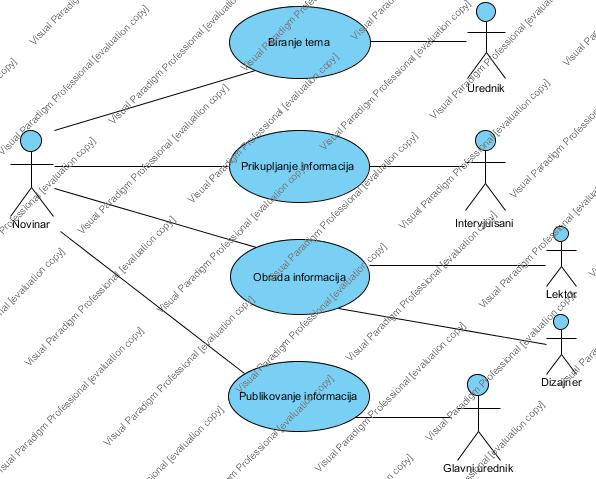
\includegraphics[width=0.7\textwidth]{slike/pisanje}
    \caption{Dijagram slučajeva upotrebe - pisanje članka}
    \label{pisanje}
\end{figure}

\subsection{Biranje tema (kolegijum)}

\begin{description}
\item [Opis] Novinari i urednici se dogovaraju oko tema koje će biti obrađene.
\item [Učesnici] Novinar, Urednik.
\item [Ulaz] Nema.
\item [Izlaz] Odabrane i dodeljene teme novinarima.
\item [Preduslovi] Dolazak dovoljnog broj novinara i urednika potrebnih za održavanje kolegijuma, prisustvo dovoljnog broj  novinara i urednika iz svake redakcije na kolegijumu.
\item [Postuslov] Uspešno odabrane i podeljene teme.
\end{description}      

\subsubsection{Glavni tok}
Urednici otpočinju kolegijum predstavljajući novinarima aktuelne teme i rezultate izvršenih analiza tržišta. Nakon izlaganja urednici daju reč novinarima. Novinar na osnovu svojih želja predlaže teme i traži odobrenje za istraživanje od urednika. Urednici zatim diskutuju o predloženim temama. Ukoliko se novinareve trenutne želje ne uklapaju sa vizijom urednika, urednici daju zadatke novinarima. Ukoliko se želje uklapaju u viziju urednika novinarev predlog se prihvata.
\subsubsection{Alternativni tok}
Ukoliko je potreban veći broj tema ili obrađivanje neke usko specijalizovane teme angažuju se honorarni novinari

\subsection{Prikupljanje informacija}
\begin{description}
\item [Opis] Novinar istražuje temu i piše prvu ruku članka.
\item [Učesnici] Novinar, Intervjuisani.
\item [Ulaz] Odabrane teme.
\item [Izlaz] Sirov(neobrađen) tekst.
\item [Preduslov] Ukoliko novinar vrši intervju, intervjuisana osoba je pristala na intervju.
\item [Postuslov] Tekst je uspešno napisan.
\end{description}      
\subsubsection{Glavni tok}
Novinar pregleda dobijene teme. Tema može da zahteva intervju, prevođenje ili samostalno istraživanje. Ukoliko tema zahteva intervju novinar zove osobu koju treba da intervjuiše. Intervjuisani u dogovoru sa novinarom može da prihvati ili odbije intervju. Ako je odbio intervju novinara, unosi u tekst informacije sa konstatacijom da intervju nije izvršen. Ukoliko prihvati intervju dogovara se sa novinarom o lokaciji i vremenu intervjua. Kada dodje na intervju novinar mu postavlja pitanja i snima odgovore. Kad se intervju završi novinar sa snimka zapisuje najzanimljivije. Ukoliko tema zahteva prevodjenje novinar preuzima tekst i prevodi ga. Ukoliko tema zahteva samostalno istraživanje novinar prikuplja literaturu, ako je potrebno organizuje neke manje intervjue. Na kraju iz hrpe prikupljenih informacija vadi najbitnije i zapisuje. 
\subsubsection{Alternativni tok}
U slučaju da kandidat odbije intervju, a drugi kandidat prihvati novinar može zanemariti prvog kandidata. 


\subsection{Obrada informacija}
\begin{description}
\item [Opis] Novinar, Lektor i Urednik proveravaju ispravnost članka.
\item [Učesnici] Novinar, Lektor, Urednik, Dizajner.
\item [Ulaz] Sirov(neobrađen) tekst.
\item [Izlaz] Tekst spreman za završnu obradu.
\item [Preduslov] Novinar je napisao neobrađeni tekst.
\item [Postuslov] Tekst je lektorisan i spreman za publikovanje.
\end{description}      
\subsubsection{Glavni tok}
Novinar čita tekst koji je napisao i važne delove, eventualno dopunjuje, u kontekstu onog što je trenutno aktuelno tj. onog što je vest. Kada je završio posao novinar predaje neobrađeni tekst lektoru. Lektor čita tekst i ukoliko primeti neke pravopisne, gramatičke i stilske greške vrši korekciju teksta. Čitanje i lektorisanje jednog teksta se vrši više puta. Kada je lektorisanje završeno, tekst se šalje uredniku da proveri istinitost konsultovanjem arhive ili više izvora. Ako je tekst istinit urednik ga odobrava u suprotnom tekst se odbacuje. Odobreni tekst salje se dizajneru koji dodaje slike, vrši prelome i stara se da tekst bude primamljiv oku. Kada je završio dizajner vraća tekst novinaru.
\subsubsection{Alternativni tok}
U borbi za čitaoce urednik se trudi da se informacija što pre objavi, pa se često preskaču koraci provere informacija i dolazi do objavljivanja neistinitih informacija.

\subsection{Publikovanje informacija}
\begin{description}
\item [Opis] Glavni urednik odobrava članak.
\item [Učesnici] Novinar, Glavni urednik.
\item [Ulaz] Obrađen tekst.
\item [Izlaz] Tekst spreman za objavljivanje i štampanje.
\item [Preduslov] Tekst je poslat uredniku.
\item [Postuslov] Tekst je odobrio urednik.
\end{description}      
\subsubsection{Glavni tok}
Novinar pregleda tekstove a zatim šalje tekst glavnom uredniku na odobrenje. Glavni urednik čita i analizira tekst. Ako glavni urednik nema zamerki, tekst dobija odobrenje da se šalje na internet objavljivanje i štampu. Ukoliko glavni urednik ima zamerki, tekst se šalje novinaru koji ga je pisao sa spiskom šta je potrebno da se uskladi. Upit može biti takav da se cenzuriše deo, čitav članak ili samo da se nešto doda. Ako je potrebno još dodati podataka ili novinar se vraća sa uputima urednika na koraka 3.1.2. Ako se cenzuriše čitav članak novinar odbacuje tekst, a ako se cenzuriše deo ide se na korak 3.1.3.
\subsubsection{Alternativni tok}
Ukoliko je ceo članak cenzurisan novinar može da pokuša da članak predstavi na sledećem kolegijumu 

	

\begin{figure}[h]
    \centering
    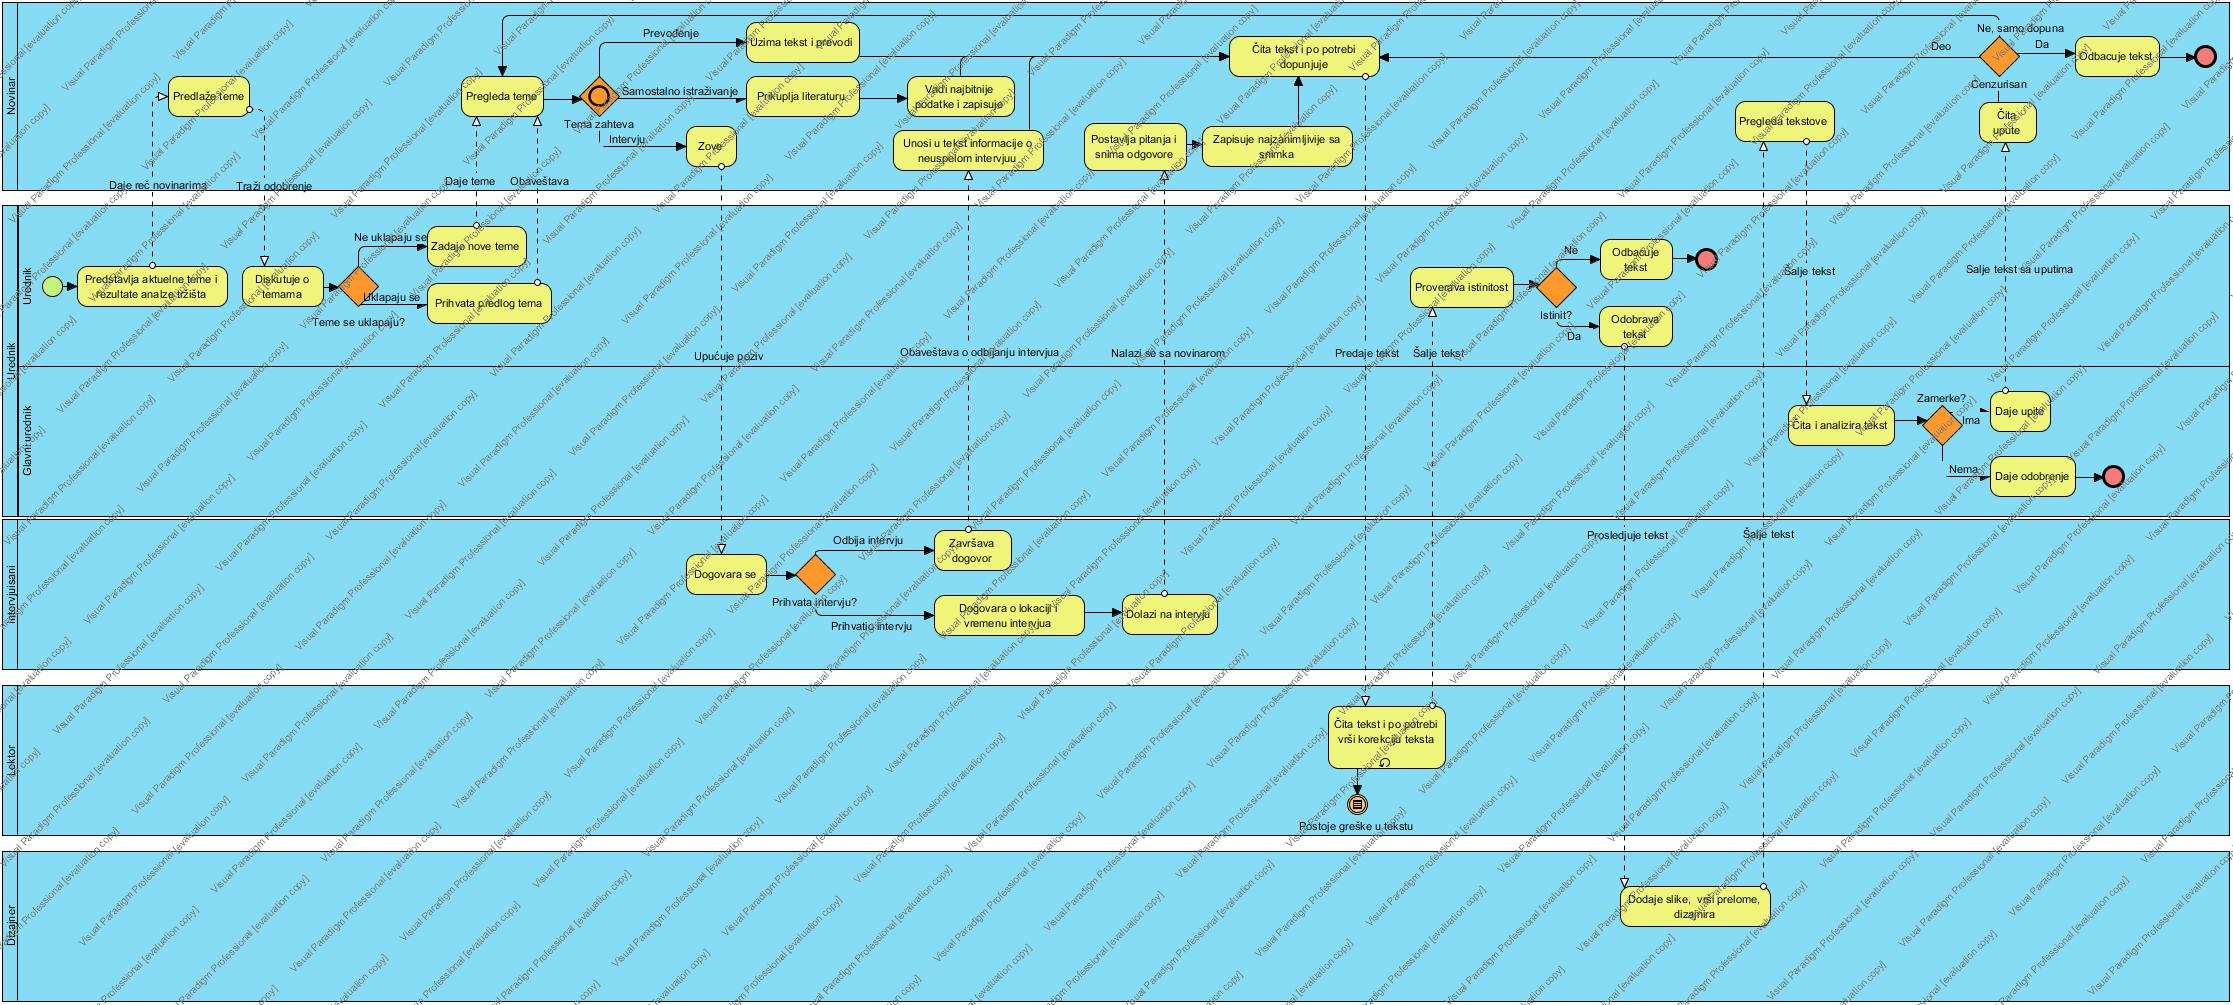
\includegraphics[width=1.0\textwidth]{slike/1-bpmn}
    \caption{BPMN dijagram}
    \label{pisanje}
\end{figure}	


.

\subsection{Komponovanje izdanja}
Za svako izdanje glavni i odgovorni urednik odlučuje o broju članaka. Takođe pored broja članaka se zna koliko kolor, a koliko crno-belih strana može izdanje da ima, kao i gde i koliko može oglasa da se nalazi. Nazalost pošto se danas novine i časopisi ne finansiraju samo od prodatih primeraka ili pretplatnika, već uglavnom od sponzora, za svakog novog sponzora, olgašivača mora da se nađe mesto, makar i na štetu kvaliteta sadržaja.

\subsubsection{Odabir članaka}
\begin{description}
\item [Opis] Glavni urednik bira članke koji će biti objavljeni.
\item [Učesnici] Glavni urednik.
\item [Ulaz] Članak spreman za objavljivanje i štampanje.
\item [Izlaz] Odabrani članci.
\item [Preduslov] Članak je spreman za objavljivanje i štampanje.
\item [Postuslov] Članak je poslat na štampu.
\end{description}   
\subsubsection{Glavni tok}
Glavni urednik pregleda članke. Pregled se sastoji od procene dužine, broja i kolora članaka. Ukoliko je broj, dužina ili kolor članaka veća od planirane vrši se odabir članaka. Ukoliko članci zadovoljavaju uslove, šalju se dalje na pripremu za štampu. Odabir članaka se vrši tako što prednost imaju aktuelne teme. 
\subsubsection{Alternativni tok}
Ukoliko je problem kolorit a sve teme su izuzetno aktuelne dozvoljava se u kontaktu sa menadžmentom da se prekorači dozvoljeni kolorit za najviše 5%.

\subsubsection{Smeštanje oglasa}
\begin{description}
\item [Opis] Glavni urednik smešta oglase u časopis.
\item [Učesnici] Glavni urednik, Oglašivač, Menadžment.
\item [Ulaz] Plaćeni oglasi.
\item [Izlaz] Raspoređeni oglasi.
\item [Preduslov] Oglašivač je platio mesto za oglas(e).
\item [Postuslov] Oglasi se nalaze na internet i/ili stampanom izdanju.
\end{description}   
\subsubsection{Glavni tok}
Glavni urednik sortira oglase prema važnosti (redovni sponzori, vanredni…). Kada je završio sa sortiranjem, urednik raspoređuje oglase prema veličini na unapred odabrane lokacije u časopisu. Ukoliko nema viška oglasa glavni urednik salje oglase na objavljivanje. Ukoliko ima više oglasa nego lokacija glavni urednik obaveštava menadžment koji onda kontaktira oglašivača. Oglašivač odlučuje da li će dodatno doplatiti da se njegov oglas nadje u časopisu na dodatnim stranama po unapred utvrđenom cenovniku ili će odustati. Ukoliko oglašivač prihvati ponudu, kad uplati sredstva kontaktira menadžment koji proverava uplatu i kontaktira glavnog urednika. Glavni urednik zatim izdaje naređenje da se oglas stavi na dodatnu stranu ili da se neki članak ukloni i na njegovo mesto dođe oglas. Ukoliko oglašivač odustane kontaktira se menadžment sa kojim se dogovara oko povraćaja novca
\subsubsection{Alternativni tok}
Ukoliko nema dovoljno oglasa raspisuje se kratkotrajni tender za prostor po smanjenoj ceni.

	
\begin{figure}[h]
    \centering
    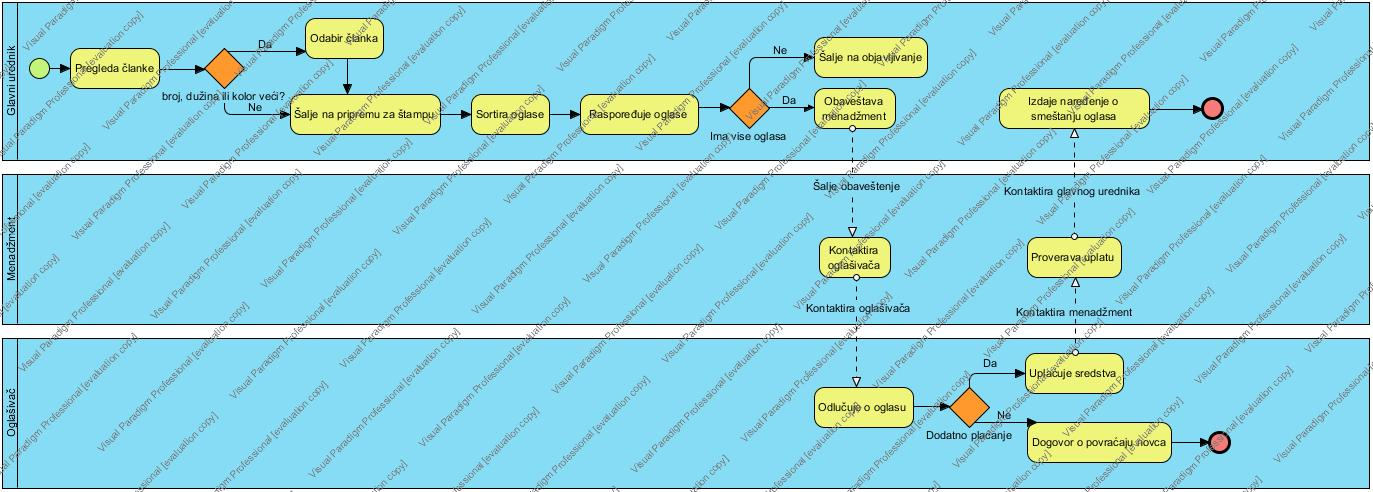
\includegraphics[width=1.0\textwidth]{slike/2-bpmn}
    \caption{BPMN dijagram}
    \label{pisanje}
\end{figure}	
\newpage

\input{./komponovanje_slucajevi.tex}
\newpage

\section{Vizuelizacija i grafički dizajn}
Iako je tekst glavni sadržaj jednog časopisa, on mora biti i vizuelno privlačan čitaocima. Zbog toga časopis ima i grafički odsek u kome su zaposleni ljudi vični krojenju izgleda kako štampanih tako i digitalnih strana. \\

Pored fotografa i ilustratora koji stvaraju potpuno nove slike iz ničega, u grafičkom odseku rade i dizajneri; profesionalci koji uklapanjem celina, izborom boja i tipografije prave prikaz na čije elemente većina čitaoca ne obraća pažnju ali koji igra ogromnu ulogu u ostavljenom utisku. \\

Celim odeskom rukovodi grafički urednik koji je osoba istančanog osećaja za izgled i dizajn. Njegova uloga je prvenstveno kritička, sav vizuelni materijal koji se u izdavaštvu proizvede on mora odobriti, on mora znati kako da d\^{a} pravi savet koji će pomoći stvaraocu da dovede svoj rad na nivo prihvatljiv standardima časopisa.


\subsection{Dizajniranje štampanog članka}
\begin{description}
\item [Opis] Grafički urednik sa svojim saradnicima kreira i određuje kako će članak u štampanom izdanju izgledati.
\item [Učesnici] (Grafički) urednik, dizajner, ilustrator (fotograf).
\item [Ulaz] Članak u tekstualnom obliku.
\item [Izlaz] Članak ukrašen i ukomponovan sa ostatkom izdanja.
\item [Preduslov] Članak je napisan i neće trpeti veće promene nadalje.
\item [Postuslov] Izgled članka je određen.
\end{description}
\subsubsection{Glavni tok}
\begin{enumerate} 
\item Urednik prima tekst članka.
\item Urednik zadužuje dizajnera za rad na članku, dajući mu predloge ukoliko ih ima.
\item Dizajner bira sliku kojom će ilustrovati članak. Pred njim su tri izbora:
\begin{enumerate}
\item Može upotrebiti sliku koja već postoji u bazi podataka.
\item Može zadužiti ilustratora (ili fotografa) da proizvede željenu sliku.
\item Može naći sliku drugde i zatražiti pravnom odseku (menadžmentu) da je licencira.
\end{enumerate}
\item Dizajner prilagođava sliku potrebama članka,
uklapa je prostorno i stvara celokupan izgled stranica na kojima će se nalaziti članak.
\item Dizajner predaje svoj rad uredniku koji ili:
\begin{enumerate}
\item Odobrava predatu verziju kao završnu i dodaje je u konačnu verziju izdanja.
\item Ili nudi kritiku dizajneru i vraća ga na korak 3 ili korak 4 ukoliko je zamerka manja.
\end{enumerate}
\end{enumerate}
\subsubsection{Alternativni tok}
Ukoliko usred prevelikog obima posla ili tehničkih nemogućnosti ilustratori (fotografi) zaposleni u izdavaštvu ne mogu napraviti željenu sliku, unajmljuje se hororarni ilustrator (fotograf).

\subsection{Dizajniranje internet članka}
\begin{description}
\item [Opis] Grafički urednik sa svojim saradnicima kreira i određuje kako će članak u štampanom izdanju izgledati.
\item [Učesnici] (Grafički) urednik, dizajner, ilustrator (fotograf).
\item [Ulaz] Članak u tekstualnom obliku.
\item [Izlaz] Ilustrovani članak u internet izdanju.
\item [Preduslov] Članak je napisan i neće trpeti veće promene nadalje.
\item [Postuslov] Izgled članka je određen.
\end{description}
\subsubsection{Glavni tok}
\begin{enumerate} 
\item Urednik prima tekst članka.
\item Urednik zadužuje dizajnera za rad na članku, dajući mu predloge ukoliko ih ima.
\item Dizajner bira sliku kojom će ilustrovati članak. Pred njim su tri izbora:
\begin{enumerate}
\item Može upotrebiti sliku koja već postoji u bazi podataka.
\item Može zadužiti ilustratora (ili fotografa) da proizvede željenu sliku.
\item Može naći sliku drugde i zatražiti pravnom odseku (menadžmentu) da je licencira.
\end{enumerate}
\item Dizajner prilagođava sliku potrebama članka, bira gde će se u tekstu nalaziti.
\item Dizajner predaje svoj rad uredniku koji ili:
\begin{enumerate}
\item Odobrava predatu verziju kao završnu i prosleđuje je administratoru koji objavljuje članak na veb stranici.
\item Ili nudi kritiku dizajneru i vraća ga na korak 3.
\end{enumerate}
\end{enumerate}
\subsubsection{Alternativni tok}
Ukoliko usred prevelikog obima posla ili tehničkih nemogućnosti ilustratori (fotografi) zaposleni u izdavaštvu ne mogu napraviti željenu sliku, unajmljuje se hororarni ilustrator (fotograf).

\subsection{Promena stila veb sajta}
\begin{description}
\item [Opis] Grafički urednik sa svojim saradnicima menja izgled sajta časopisa.
\item [Učesnici] (Grafički) urednik, dizajner, administrator.
\item [Ulaz] Trenutni izgled sajta (.css dokument).
\item [Izlaz] Novi izgled sajta (.css dokument).
\item [Preduslov] Sajt radi normalno.
\item [Postuslov] Sajt radi isto, ima novi izgled.
\end{description}
\subsubsection{Glavni tok}
\begin{enumerate} 
\item Urednik osmišlja novi izgled sajta.
\item Urednik predočava svoju zamisao dizajneru.
\item Dizajner određuje elemente stila, geometriju, boje, tipografiju. Pravi manje slike koje se koriste kao ikonice.
\item Dizajner predaje svoj rad uredniku koji ili:
\begin{enumerate}
\item Odobrava i predaje rezultat administratoru koji ga podešava kao novi izgled stranice.
\item Ili nudi kritiku dizajneru i vraća ga na korak 3.
\end{enumerate}
\end{enumerate}
\subsubsection{Alternativni tok}
Ukoliko promene dovedu do nepredviđenih problema kasnije, stari stil se može privremeno vratiti dok se rešenje ne nađe.

\subsection{Dizajn naslovne strane}
\begin{description}
\item [Opis] Uredništvo zajedno sa dizajnerima osmišlja i kreira naslovnu stranu štampanog izdanja.
\item [Učesnici] Glavni urednik, Grafički urednik, ostali urednici, dizajneri.
\item [Ulaz] Nema.
\item [Izlaz] Naslovna strana.
\item [Preduslov] Sadržaj novog izdanja je okvirno poznat.
\item [Postuslov] Naslovna strana za iduće izdanje je napravljena.
\end{description}
\subsubsection{Glavni tok}
\begin{enumerate} 
\item Uredništvo (Glavni i grafički sa izvršnim urednicima) se okuplja i razmenjuje ideje za naslovnu stranu,
 uključujući pored slike koja će biti prikazana i koji članci će biti promovisani na njoj.
\item Glavni urednik bira najbolju od predloženih ideja.
\item Grafički urednik nadograđuje ideju detaljima za koje misli da bi načinili bolju sliku i zadužuje grafičke radnike da rade na njoj.
\item Nabavlja se osnovna slika tako što:
\begin{enumerate}
\item Ilustrator stvara sliku bilo ručno ili pomoću programa ili u nekoj kombinaciji.
\item Fotograf slika osobu, predmet ili prizor koji je zatražen.
\item Licencira se već postojeća slika.
\end{enumerate}
\item Dizajner dodaje promotivne naslove članaka, usklađuje boje i slično i predaje svoj rad grafičkom uredniku koji:
\begin{enumerate}
\item Odobrava i predaje rezultat glavnom uredniku.
\item Ili nudi kritiku dizajneru i vraća ga na korak 3.
\end{enumerate}
\item Glavni urednik isto tako kritikuje ili odobrava, ukoliko je odobreno to se smatra konačnom verzijom i biva štampano sa ostatkom izdanja. 
\end{enumerate}
\subsubsection{Alternativni tok}
U nedostatku prihvatljivih ideja od strane uredništva, grafičkom odseku se može dati veća kreativna sloboda pri kreiranju stranice. Ova svejedno mora proći kroz odobrenje grafičkog i glavnog urednika.

\subsection{Pravljenje fotoportreta}
\begin{description}
\item [Opis] Fotograf pravi fotografiju osobe.
\item [Učesnici] Fotograf, fotografisani (često intervjuisani), grafički urednik.
\item [Ulaz] Nema.
\item [Izlaz] Profesionalna fotografija osobe.
\item [Preduslov] Osoba je pristala da se slika za časopis.
\item [Postuslov] Slika je spremna da se upotrebi u časopisu.
\end{description}
\subsubsection{Glavni tok}
\begin{enumerate} 
\item Fotograf i osoba se nalaze na dogovorenom mestu: studiju ili na mestu gde je osoba intervjuisana.
\item Fotograf namešta potrebnu opremu i pravi niz fotografija sa osobom.
\item Fotograf sa grafičkim urednikom bira najpogodniju fotografiju iz niza.
\end{enumerate}
\subsubsection{Alternativni tokovi}
\begin{enumerate} 
\item Ukoliko osoba povuče svoj pristanak u bilo kom momentu posao se obustavlja.
\item Ukoliko nijedna fotografija nije prihvatljiva slikanje se može ponoviti, mada se ovo izbegava jer bi bilo neprijatno za osobu koja se slika.
\end{enumerate}

\subsection{Licenciranje slike}
\begin{description}
\item [Opis] Administracija se na zahtev grafičkog dizajnera dogovara sa vlasnikom licence da otkupi prava na upotrebu slike.
\item [Učesnici] Dizajner, Menadžer, vlasnik.
\item [Ulaz] Nema.
\item [Izlaz] Zvanična dozvola za upotrebu slike.
\item [Preduslov] Dizajner zna koja mu je slika potrebna i vlasnik prava se može naći.
\item [Postuslov] Časopis može legalno koristiti sliku.
\end{description}
\subsubsection{Glavni tok}
\begin{enumerate} 
\item Grafički dizajner nalazi sliku koja mu je potrebna
\item 
\end{enumerate}
\subsubsection{Alternativni tok}
Ukoliko usred prevelikog obima posla ili tehničkih nemogućnosti ilustratori (fotografi) zaposleni u izdavaštvu ne mogu napraviti željenu sliku, unajmljuje se hororarni ilustrator (fotograf).
\newpage

\section{Odabir saradnika}
Kao i svakoj organizaciji ili preduzeću, časopisu je potrebna procedura zapošljavanja radnika. Iako je ovo donekle administrativno pitanje, u kreativnom poslu kao što je stvaranje članaka posebno je bitno da se saradnici međusobno uklapaju te stoga u ovom poslu uredništvo takođe ima veoma aktivnu ulogu.


\subsection{Raspis konkursa}
\begin{description}
\item [Opis] Zahtev za novim radnikom (ili radnicima) se prosleđuje do administracije koja raspisuje konkurs.
\item [Učesnici] Urednik (izvršni ili grafički), glavni urednik, administracija.
\item [Ulaz] Nema.
\item [Izlaz] Konkurs za zapošljavanje.
\item [Preduslov] Postoji potreba za dodatnim saradnicima.
\item [Postuslov] Konkurs je raspisan.
\end{description}
\subsubsection{Glavni tok}
\begin{enumerate} 
\item Urednik obaveštava glavnog urednika o potrebi za dodatnim radnikom (kolumnistom, izveštačem, dizajnerom, fotografom,...).
\item Glavni urednik razmotri situaciju i podnese zahtev administraciji.
\item Administracija sastavlja konkurs na osnovu datih podataka i u skladu sa zakonom.
\item Administracija objavljuje konkurs.
\end{enumerate}
\subsubsection{Alternativni tokovi}
\begin{enumerate} 
\item Ukoliko glavni urednik zaključi da ipak nema potrebe za novim saradnicima, tok se obustavlja.
\item Ukoliko administracija nema dovoljno sredstava ili smatra da trošak nije opravdan obustavlja se tok.
\item Ukoliko postoji neka ranije intervjuisana osoba koja bi dobro odgovarala potrebama ona se obaveštava o konkursu.
\end{enumerate}

\subsection{Intervju potencijalnog saradnika}
\begin{description}
\item [Opis] Urednik razgovara sa kandidatom da bi ocenio koliko je pogodan kao saradnik.
\item [Učesnici] Urednik (izvršni ili grafički), kandidat.
\item [Ulaz] Uzorak kandidatovog prethodnog rada.
\item [Izlaz] Izveštaj o kandidatu.
\item [Preduslov] Kandidat se prijavio na konkurs i zainteresovan je za saradnju.
\item [Postuslov] Urednik je stekao uvid u kandidatove sposobnosti i ličnost.
\end{description}
\subsubsection{Glavni tok}
\begin{enumerate} 
\item Urednik se dogovara sa kandidatom oko mesta i vremena kada će se intervju održati.
\item Kandidat i urednik se nalaze i urednik razgovara sa kandidatom, postavljajući mu pitanja koja se odnose na njegove kvalifikacije, kandidat daje uredniku neke primere svog pređašnjeg rada.
\item Kandidat odlazi, urednik gleda uzorke njegovog rada i piše izveštaj sa podacima o kandidatu i oceni njegove pogodnosti.
\end{enumerate}
\subsubsection{Alternativni tokovi}
\begin{enumerate} 
\item Ako se tako odluči, Kandidat može obustaviti intervju u svakom momentu.
\item Zakazani sastanak može se pomeriti ukoliko to postane neophodno za nekog od učesnika.
\item Kandidat može poslati uzorke svog rada umesto što ih lično donosi.
\end{enumerate}

\subsection{Zapošljavanje kandidata}
\begin{description}
\item [Opis] Uredništvo odlučuje kog od intervjuisanih kandidata će zaposliti.
\item [Učesnici] Glavni urednik, ostali urednici, administracija, kandidat
\item [Ulaz] Izveštaji o kandidatima.
\item [Izlaz] Nema.
\item [Preduslov] Postoji makar jedan kandidat.
\item [Postuslov] Kandidat je izabran.
\end{description}
\subsubsection{Glavni tok}
\begin{enumerate} 
\item Redakcija se okuplja i diskutuje o kandidatima na osnovu izveštaja. 
\item Kandidat se bira ili jednoglasno ili, ako to nije moguće, po izboru glavnog odgovornog urednika.
\item Kandidat se kontaktira i administracija obavlja formalnosti zapošljavanja .
\end{enumerate}

\newpage

\section{Izdavanje}
Predstavlja završnu fazu procesa izrade novog izdanja časopisa.

Finalizovana verzija u ovom obliku se naposletku dostavlja čitaocu u štampanom ili pak elektronskom izdanju.

\subsection{Izbor štamparije}
\begin{description}
\item [Opis] Menadžment vrši odabir štamparije koja će biti zadužena za štampanje izdanja čaopisa.
\item [Učesnici] Menadžment, štamparija.
\item [Preduslov] Uspešno izvršene faze koje prethode izdavanju.
\item [Postuslov] Primerci časopisa spremni za distribuciju.
\end{description}
\subsubsection{Glavni tok}
Menadžment vrši inicijalnu pretragu mogućih štamparija kod kojih bi tražili uslugu. Uzimajući u obzir geografsku lokaciju zbog kasnijeg distribuiranja, menadžment sužava izbor i kontaktira određene štamparije.
Za svaku od štamparija proverava kvalitet štampe i cenu štampanja. Menadžment potom pravi izbor štamparije i dostavlja joj finalnu verziju izdanja, gde pritom naglašava broj primeraka koji želi da štampa.
Štamparija potom obaveštava menadžment pošto završi proces štampanja.

\subsection{Isporuka štampanog izdanja}
\begin{description}
\item [Opis] Dostava štampanog izdanja do prodajnog mesta.
\item [Učesnici] Štampar, distributer, menadžment.
\item [Preduslov] Ištampani primerci časopisa.
\item [Postuslov] Primerci dosavljeni do prodajnog mesta.
\end{description}
\subsubsection{Glavni tok}
Štamparija dostavlja distributeru primerke časopisa. Menadžment dostavlja spisak maloprodajnih objekata distrubuteru koji potom određuje optimalnu rutu isporuke primeraka časopisa. Po uspešnoj distribuciji distributer dobija novčanu naknadu od menadžmenta.

\subsection{Objavljivanje online izdanja}
\begin{description}
\item [Opis] Predstavlja izmenu web strane online izdanja na trenutno izdanje
\item [Učesnici] Administrator, glavni urednik
\item [Ulaz] Trenutni izgled sajta (.css dokument).
\item [Izlaz] Novi izgled sajta (.css dokument).
\item [Preduslov] Uspešno izvršene sve faze koje prethode izdavanju.
\item [Postuslov] Nova online verzija uspešno postavljena na web strani časopisa.
\end{description}
\subsubsection{Glavni tok}
Glavni urednik dostavlja finalnu verziju administratoru. Administrator analizira izdanje i prilagođava finalnu verziju web prezentaciji izdanja; potom vrši potrebne korake kako bi izdanje učinio dostupnim na webu.
Potom vrši nadgledanje web strane zbog eventualnih izmena koje mogu biti neophodne u budućnosti. Takođe za pretplaćene korisnike omogućuje dostupnim dodatni sadržaj.

\newpage

\section{Oglašavanje}
Oglašavanje predstavlja vid saradnje između časopisa i zakupca oglasnog prostora. To je mogućnost za zakupca da putem oglasa u časopisu promoviše svoj proizvod ili uslugu, dok sa druge strane predstavlja materijalnu dobit za časopis.

Imajući u vidu obostranu korist, oglasni prostor je skoro uvek obavezan u sastavu jednog časopisa.

\subsection{Određivanje cene oglasnog prostora}
\begin{description}
\item [Opis] Podela oglasnog prostora prema cenovnom rangu.
\item [Učesnici] Menadžment.
\item [Preduslov] Određene pozicije oglasa u časopisu.
\item [Postuslov] Oglasni prostor kategorisan prema ceni.
\end{description}
\subsubsection{Glavni tok}
Menadžment zajedno sa glavnim urednikom analizira postojeće sekcije u časopisu. Prema njihovoj aktuelnosti, određuje cenu prostora za oglas koji pripada sekciji.
Cena može biti korigovana u budućnosti u zavisnosti od ponude i potražnje.

\subsection{Zakupljivanje oglasnog prostora}
\begin{description}
\item [Opis] Postizanje dogovora između menadžmenta i zakupca oglasnog prostora.
\item [Učesnici] Zakupac oglasa, menadžment.
\item [Preduslov] Definisan prostor u časopisu predviđen za oglae kao i njegova cena
\item [Postuslov] Uspešno prodat oglasni prostor.
\end{description}
\subsubsection{Glavni tok}
Zakupac kontaktira menadžment kako bi se informisao o cenama oglasa. Menadžment saopštava cene oglasnog prostora po kategorijama.
Zakupac shodno svojim željama i finansijkim mogućnostima pravi izbor, saopštava menadžmentu onaj prostor koji je voljan da zakupi. Potom šalje oglase menadžmentu koje želi da objavi. Eventualno se pretplaćuje na oglasni prostor na duži vremenski period.
Menadžment i zakupac formalno sklapaju ugovor o zakupljenom oglasnom prostoru.

\newpage

\section{Pretplata}
Predstavlja jedan način podrške časopisa od strane čitalaca. Jedna od prednosti je dobijanje izdanja po povoljnijoj ceni u poređenju sa kupovanjem pojedninačnih primeraka. 

Druga pogodnost je da će časopis biti dostavljen na kućnu adresu čitaoca. Takođe, ne postoji bojazan da bi čitaloci mogli da zaborave da kupe mesečno izdanje časopisa usled nedostatka vremena ili odsustva.

\subsection{Osmišljanje modela pretplate}
\begin{description}
\item [Opis] Menadžment razmatra različite tipove pretplate sa stanovišta perioda i cene pretplate.
\item [Učesnici] Menadžment.
\item [Preduslov] Nema.
\item [Postuslov] Definisani jedan ili više modela pretplate.
\end{description}
\subsubsection{Glavni tok}
Menadžment postavlja okvire cene i perioda nad kojima se vrši pretplata. Uzimaju se u obzir uobičajeni vremenski periodi na koje bi se davala pretplata(npr. 6m, 1g, 2g) kao i odgovarajuća cena.
Ukoliko se časopis ne izdaje u intervalima od jednog meseca, pretplata se zasniva na broju primeraka. Menadžment dalje odlučuje za svaki predloženi model pretplate dodatne pogodnosti kojima će nagraditi pretplatnike.
Vrši se odabir jednog ili više predloženih modela pretplate.

\subsection{Ugovaranje pretplate}
\begin{description}
\item [Opis] Čitalac kontaktira menadžment časopisa radi pretplate.
\item [Učesnici] Čitalac, menadžment.
\item [Ulaz] Kontakt čitaoca.
\item [Izlaz] Izvršena pretplata.
\item [Preduslov] Časopis ima definisane modele pretplate.
\item [Postuslov] Čitalac se uspešno pretplatio.
\end{description}
\subsubsection{Glavni tok}
Menadžment pre isporuke novog izdanja na prodajna mesta kontaktira distributera. Pre toga dohvata informacije o adresama stanovanja pretplatnika i prosleđuje ih distributeru. 
Distributer, zajedno sa primercima časopisa i podacima o adresama vrši isporuku.
\subsubsection{Alternativni tok}
Ukoliko čitalac iz određenih okolnosti odluči da prekine pretplatu, to saopštava menadžmentu i vrši se delimični povraćaj novca.

\begin{figure}[ht]
    \centering
    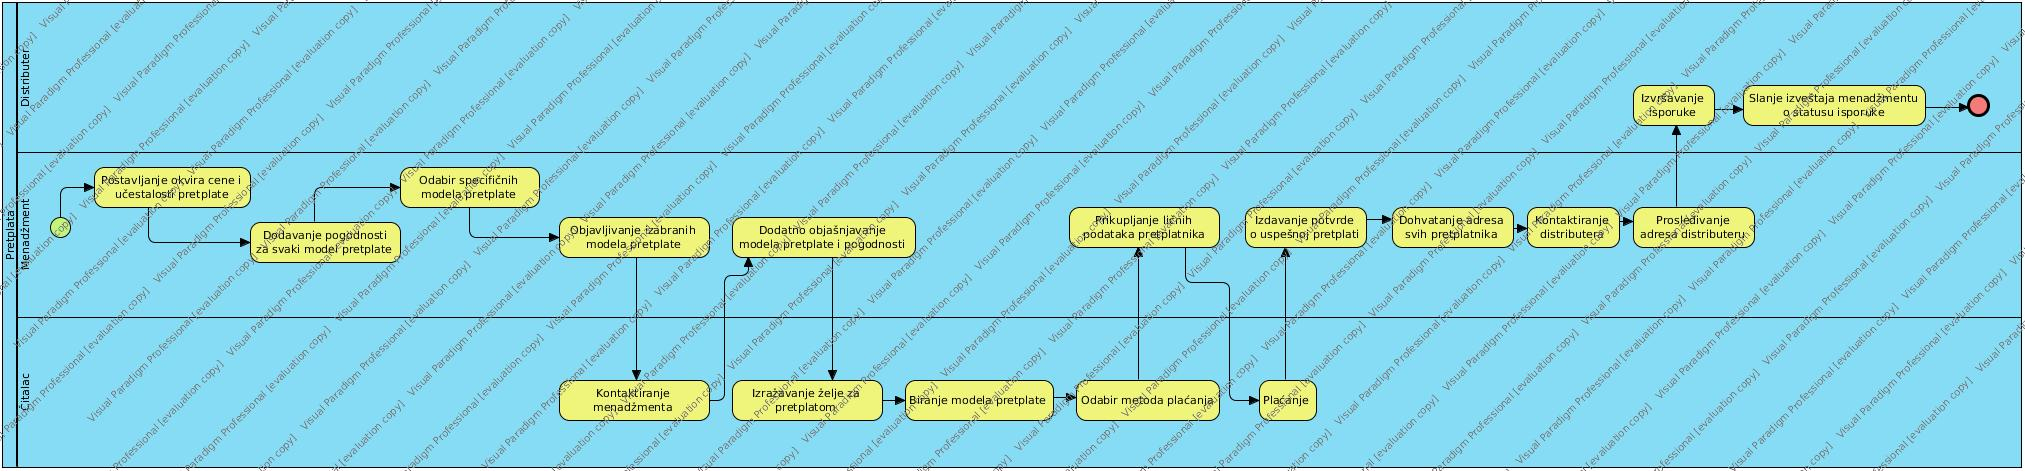
\includegraphics[width=0.9\textheight, angle=90]{slike/pretplata}
    \caption{BPMN dijagram - Pretplata}
    \label{pretplata}
\end{figure}

\subsection{Distribucija časopisa pretplatnicima}
\begin{description}
\item [Opis] Menadžment organizuje dostavu časopisa pretplatnicima.
\item [Učesnici] Menadžment, distributer.
\item [Preduslov] Primerci časopisa za isporuku su ištampani.
\item [Postuslov] Časopis dostavljen na krajnju adresu čitalaca.
\end{description}
\subsubsection{Glavni tok}
Menadžment pre isporuke novog izdanja na prodajna mesta kontaktira distributera. Pre toga dohvata informacije o adresama stanovanja pretplatnika i prosleđuje ih distributeru. Distributer, zajedno sa primercima časopisa i podacima o adresama vrši isporuku.
Po uspešno izvršenoj isporuci javlja menadžmentu da li je isporuka uspešno izvršena, kako bi eventualno pretplatnici bili obavešteni o mogućim komplikacijama.



\newpage

\chapter{Klase podataka}

Razmatranjem slučajeva upotrebe zaključeno je da je za funkcionisanje informacionog sistema najbitnije čuvati sledeće podatke:
\begin{enumerate}
\item Podaci o zaposlenima
\item Podaci o slikama
\item Podaci o autorstvu
\item Podaci o izdanjima
\item Podaci o ugovorima
\item Podaci o konkursima
\end{enumerate}

\begin{figure}[htp]
    \centering
    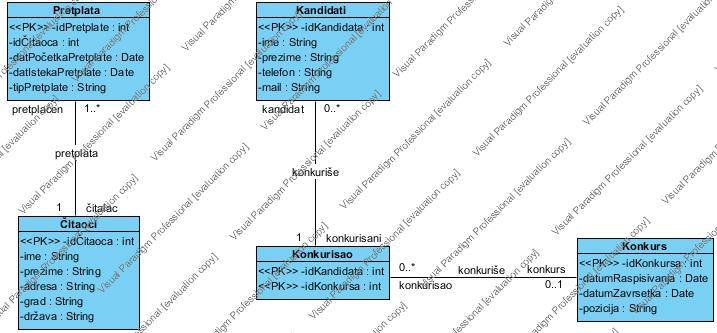
\includegraphics[width=0.9\textwidth]{slike/konkurs-pretplata}
    \caption{Klasni dijagram 1. deo}
    \label{klase1}
\end{figure}    

\begin{figure}[htp]
    \centering
    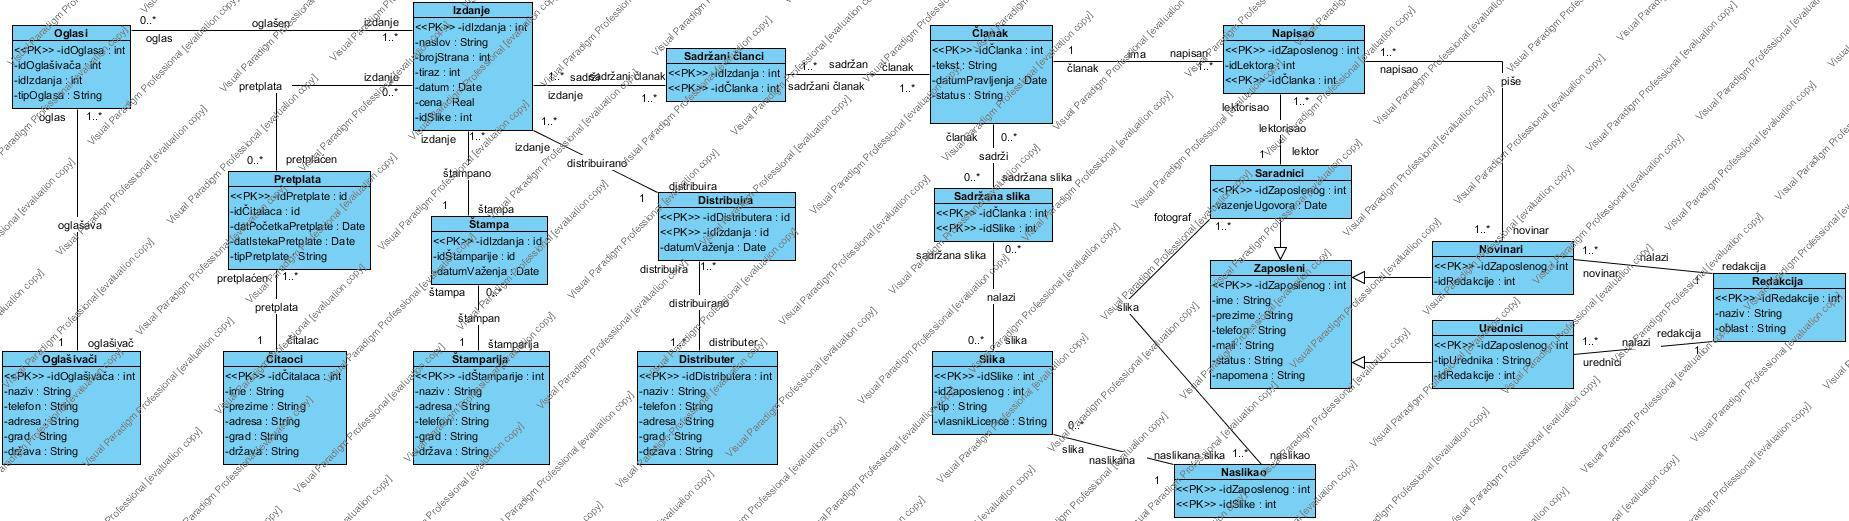
\includegraphics[width=0.9\textheight, angle=90]{slike/klasni_dijagram}
    \caption{Klasni dijagram 2. deo}
    \label{klase2}
\end{figure}    



\newpage

\section{Podaci o zaposlenima}
Klasa \textbf{zaposleni} i klase koje se izvode iz nje su ključni deo informacionog sistema. Klase koje su izvedene su \textbf{urednik}, \textbf{novinar} i \textbf{saradnik}. One preuzimaju sve atribute iz roditeljske klase i dodaju sebi specifične. \\

Kod \textbf{urednik} to je tip urednika i identifikacija redakcije kojoj urednik pripada, kod \textbf{novinar}  to je  identifikacija redakcije kojoj novinar pripada, kod \textbf{saradnik} to je podatak do kad saradnik ima važeći ugovor sa izdavaštvom. \vspace{5mm}

\noindent \textbf{Zaposleni}
\begin{enumerate}
\item Identifikacioni broj zaposlenog (PK)
\item Ime
\item Prezime
\item Telefon
\item Adresa
\item  Imejl
\item Status (može biti "stalni", "honorarni" ili "bivši")
\item Napomena (za dodatne informacije)
\end{enumerate} \vspace{5mm}

\noindent \textbf{Urednik}
\begin{enumerate}
\item Identifikacioni broj zaposlenog (PK/SK)
\item Tip urednika (može biti "glavni", "obični" ili "grafički")
\item Identifikacioni broj redakcije (SK)
\end{enumerate} \vspace{5mm}

\noindent \textbf{Novinar}
\begin{enumerate}
\item Identifikacioni broj zaposlenog (PK/SK)
\item Identifikacioni broj redakcije (SK)
\end{enumerate} \vspace{5mm}

\noindent \textbf{Saradnik}
\begin{enumerate}
\item Identifikacioni broj zaposlenog (PK/SK)
\item Važenje ugovora (mora biti Null za stalne saradnike)
\end{enumerate} \vspace{5mm}

\section{Podaci o slikama}
Klasa \textbf{slika} pamti autora slike ukoliko ju je zaposleni napravio, njen tip (fotografija, ilustracija) kao i vlasnika licence ukoliko je slika licencirana od nekuda. 

\noindent \textbf{Slika}
\begin{enumerate}
\item Identifikacioni broj slike (PK)
\item Identifikacioni broj saradnika koji je napravio sliku (SK)
\item Tip (fotografija ili ilustracija)
\item Vlasnik Licence
\end{enumerate} \vspace{5mm}


\section{Podaci o autorstvu}

Neki članak može biti biti napisan od jednog ili više novinara. Klasa \textbf{Napisao} čuva podatke o tome koji su novinari napisali članak i koji je lektor lektorisao tekst.

\noindent \textbf{Napisao}
\begin{enumerate}
\item Identifikacioni broj članka (PK/SK)
\item Identifikacioni broj novinara (PK/SK)
\item Identifikacioni broj Lektora (Saradnika)
\end{enumerate} \vspace{5mm}

\section{Podaci o izdanjima}
O izdanjima se čuvaju informacije o datumu izdavanja, tiražu, broju strana, ceni u dinarima, slici koja se koristi kao naslovna strana i spisku članaka koji se nalaze u okviru izdanja. Spisak članaka se nalazi u okviru klase \textbf{Sadržani članci} koja pored identifikacionig broja izdanja čuva i identifikacioni broj članka i broj strane na kojoj se dati članak pojavljuje 


\noindent \textbf{Izdanje}
\begin{enumerate}
\item Identifikacioni broj izdanja (PK)
\item Naslov
\item Broj strana
\item Tiraž
\item Datum izdavanja
\item Cena
\item Identifikacioni broj slike koja služi kao naslovna strana (SK)
\end{enumerate} \vspace{5mm}


\noindent \textbf{Sadržani članci}
\begin{enumerate}
\item Identifikacioni broj izdanja (PK/SK)
\item Identifikacioni broj članka (PK/SK)
\item Broj strane na kojoj se članak pojavljuje
\end{enumerate} \vspace{5mm}

\section{Podaci o ugovorima}
Podaci o ugovorima su oni podaci koji se odnose na saradnju sa spoljnim entitetima i same entitete. Tu spadaju:\\

\noindent \textbf{Distributeri}
\begin{enumerate}
\item Identifikacioni broj distributera (PK)
\item Naziv
\item Telefon
\item Adresae
\item Grad
\item Država
\item Dužina ugovora
\end{enumerate} \vspace{5mm}

\noindent \textbf{Distribuira}
\begin{enumerate}
\item Identifikacioni broj izdanja (PK/SK)
\item Identifikacioni broj distributera (PK/SK)
\end{enumerate} \vspace{5mm}

\noindent \textbf{Štamparije}
\begin{enumerate}
\item Identifikacioni broj štamparije (PK)
\item Naziv
\item Telefon
\item Adresa
\item Grad
\item Država
\item Dužina ugovora
\end{enumerate} \vspace{5mm}

\noindent \textbf{Štampa}
\begin{enumerate}
\item Identifikacioni broj izdanja (PK/SK)
\item Identifikacioni broj štamparije (SK)
\end{enumerate} \vspace{5mm}

\noindent \textbf{Čitaoci}
\begin{enumerate}
\item Identifikacioni broj čitaoca (PK)
\item Ime
\item Prezime
\item Telefon
\item Adresa
\item Grad
\item Država
\end{enumerate} \vspace{5mm}

\noindent \textbf{Pretplate}
\begin{enumerate}
\item Identifikacioni broj pretplate (PK)
\item Identifikacioni broj čitaoca (SK)
\item DatumPočetka
\item DatumKraja
\item TipPretplate (na pisano ili Internet izdanje)
\end{enumerate} \vspace{5mm}

\noindent \textbf{Oglašivači}
\begin{enumerate}
\item Identifikacioni broj oglašivača (PK)
\item Naziv
\item Telefon
\item Adresa
\item Grad
\item Država
\end{enumerate} \vspace{5mm}

\noindent \textbf{Oglasi}
\begin{enumerate}
\item Identifikacioni broj oglasa (PK)
\item Identifikacioni broj oglasa (SK)
\item Identifikacioni broj izdanja (SK)
\item TipOglasa
\item Strana
\end{enumerate}  \vspace{5mm}

\section{Podaci o konkursima}
Klasa \textbf{konkurs} čuva podatke o raspisanim konkursima za datu poziciju i od kad do kad traju. \textbf{Kandidat} čuva podatke o potencijalnim zaposlenima dok \textbf{konkurisao} vezuje te dve klase.

\noindent \textbf{Konkurs}
\begin{enumerate}
\item Identifikacioni broj konkursa (PK)
\item Datum raspisivanja
\item Datum završretka
\item Pozicija (za koju se konkuriše)
\item Napomena
\end{enumerate}  \vspace{5mm}

\noindent \textbf{Konkurisao}
\begin{enumerate}
\item Identifikacioni broj konkursa (PK/SK)
\item Identifikacioni broj kandidata (PK/SK)
\end{enumerate}  \vspace{5mm}


\noindent \textbf{Kandidat}
\begin{enumerate}
\item Identifikacioni broj kandidata (PK)
\item Ime
\item Prezime
\item Telefon
\item mail
\end{enumerate}  \vspace{5mm}


\newpage

\input{./zakljucak.tex}


\end{document}
